\documentclass[12pt, a4paper, oneside]{Thesis} % Paper size, default font size and one-sided paper
\usepackage{wrapfig}
\usepackage{lscape}
\usepackage{rotating}
\usepackage{graphicx}
\usepackage{caption}
\usepackage{amsmath}


\usepackage{lineno,hyperref}
\modulolinenumbers[5]


\usepackage{amssymb}
\usepackage{graphicx}
\usepackage{array}
\usepackage{float}
\usepackage{placeins}
\usepackage{stackengine}
\usepackage{url}
\usepackage{numprint}
\usepackage{caption}

\usepackage{booktabs}  
\usepackage{siunitx}
%\usepackage[showframe=false]{geometry}
\usepackage{subfigure}

\nprounddigits{3}
\newcolumntype{P}[1]{>{\centering\arraybackslash}p{#1}}
\newcolumntype{M}[1]{>{\centering\arraybackslash}m{#1}}

\setstackEOL{\#}
\setstackgap{L}{12pt}


%\usepackage{subcaption} %incompatible with subfig
\graphicspath{{Pictures/}} % Specifies the directory where pictures are stored
\usepackage{natbib} % Use the natbib reference package - read up on this to edit the reference style; if you want text (e.g. Smith et al., 2012) for the in-text references (instead of numbers), remove 'numbers' v

\hypersetup{urlcolor=black, colorlinks=false} % Colors hyperlinks in blue - change to black if annoyingv`	

\thesistitle{Learning correspondence estimation for deformable 3D shapes}
\supervisor{Professor Ayan Chaudhury}
\degree{Integrated Dual Degree (B.Tech + M.Tech)}
\degreemajor{Computer Science and Engineering}
\authors{Lubesh Kumar Sharma}
\rollno{22CS30065}
\university{Indian Institute of Technology Kharagpur}
\department{Department of Computer Science and Engineering}
\unisite{http://www.iitkgp.ac.in}
\depsite{http://www.iitkgp.ac.in/department/CSE}
\placeshrt{Kharagpur}
\placelng{Kharagpur - 721302, India}
\datesub{8 Nov 2026}
\datesig{8 Nov 2026}
\semsub{Spring Semester, 2025-26}
\keywords{Learning correspondence estimation for deformable 3D shapes}
\coursecd{Project-II (CS47006) }

\title{\ttitle} % Defines the thesis title - don't touch this
\begin{document}
%\makeatletter
%\renewcommand*{\NAT@nmfmt}[1]{\textsc{#1}}
%\makeatother

% prints author names as small caps


\frontmatter % Use roman page numbering style (i, ii, iii, iv...) for the pre-content pages

\setstretch{1.6} % Line spacing of 1.6 (double line spacing)

% Define the page headers using the FancyHdr package and set up for one-sided printing
\fancyhead{} % Clears all page headers and footers
\rhead{\thepage} % Sets the right side header to show the page number
\lhead{} % Clears the left side page header

%\pagestyle{fancy} % Finally, use the "fancy" page style to implement the FancyHdr headers

\newcommand{\HRule}{\rule{\linewidth}{0.5mm}} % New command to make the lines in the title page

% PDF meta-data
\hypersetup{pdftitle={\ttitle}}
\hypersetup{pdfsubject=\subjectname}
\hypersetup{pdfauthor=\authornames}
\hypersetup{pdfkeywords=\keywordnames}

%----------------------------------------------------------------------------------------
%	TITLE PAGE
%----------------------------------------------------------------------------------------
\maketitle
%\titlepg % Add a gap in the Contents, for aesthetics

\clearpage % Start a new page

%----------------------------------------------------------------------------------------
%	DECLARATION PAGE
%	Your institution may give you a different text to place here
%----------------------------------------------------------------------------------------


\Declaration{}% Add a gap in the Contents, for aesthetics


%----------------------------------------------------------------------------------------
%	CERTIFICATE PAGE
%----------------------------------------------------------------------------------------

\addtotoc{Certificate} % Add the "Abstract" page entry to the Contents

\certificate{\addtocontents{toc}{}} % Original certificate layout

\clearpage % Start a new page

%----------------------------------------------------------------------------------------
%	ABSTRACT PAGE
%----------------------------------------------------------------------------------------

\addtotoc{Abstract} % Add the "Abstract" page entry to the Contents

\abstract{\addtocontents{toc}{} % Add a gap in the Contents, for aesthetics

Dense correspondence between deformable three-dimensional shapes requires a dense map that preserves anatomical meaning across changes in pose and orientation. This report presents a point-cloud pipeline combining spectral geometry, relative orientation estimation, masked representation learning and deformation-guided matching. Heat-based descriptors and explicit coordinates describe each point, while an orientation module adapted from SE-ORNet predicts relative yaw through overlapping angular bins and continuous refinement. A shared Adaptive Siamese Masked Autoencoder learns geometric features through cross-shape reconstruction, supported by intrinsic consistency, self-identity supervision and confidence-weighted DINOv2 distillation.

\vspace{0.8cm}

Heat-Anchored Deformation Matching combines the learned geometric and visual features with intrinsic anchor verification, anchor-relative descriptors and non-rigid deformation. The resulting dense map supports attribute transfer between differently posed shapes. The experimental progression examines coordinate conditioning, visual cues, distortion regularization, point-estimated normals, canonicalization and relative orientation. Qualitative observations of partial left--right improvement under distortion regularization motivated further study of front--back alignment. The report describes the roles of the pipeline modules and the experimental rationale connecting them, with a concise overview following the conclusion and a detailed account in the appendix.
}

\clearpage % Start a new page



%----------------------------------------------------------------------------------------
%	ACKNOWLEDGEMENTS
%----------------------------------------------------------------------------------------

\setstretch{1.3} % Reset the line-spacing to 1.3 for body text (if it has changed)

\acknowledgements{\addtocontents{toc}{} % Add a gap in the Contents, for aesthetics

\noindent
I would like to thank my supervisor Professor Ayan Chaudhury, Department of Computer Science and Engineering, Indian Institute of Technology Kharagpur, for his valuable guidance and support throughout the course of my B.Tech project work.

\vspace{0.8cm}

\noindent
I would like to thank Mr. Supon Mazumdar, Department of Computer Science and Engineering, IIT Kharagpur, who has helped me continuously in this project. Without his tremendous support, this work might not have been completed.

\vspace{0.8cm}

\noindent
I would like to express my gratitude to all faculty members of the Department of Computer Science and Engineering for guiding us and providing knowledge in various subjects over the past few years.

\vspace{0.8cm}

\noindent
Finally, my deep and sincere gratitude to my family and friends at IIT Kharagpur for their continuous love and support.

}

\clearpage % Start a new page

%----------------------------------------------------------------------------------------
%	LIST OF CONTENTS/FIGURES PAGES
%----------------------------------------------------------------------------------------

\pagestyle{fancy} % The page style headers have been "empty" all this time, now use the "fancy" headers as defined before to bring them back

\lhead{\emph{Contents}} % Set the left side page header to "Contents"
\tableofcontents % Write out the Table of Contents

\lhead{\emph{List of Figures}} % Set the left side page header to "List of Figures"
\listoffigures % Write out the List of Figures

\lhead{\emph{List of Tables}} % Set the left side page header to "List of Tables"
\listoftables % Write out the List of Tables

%----------------------------------------------------------------------------------------
%	ABBREVIATIONS
%----------------------------------------------------------------------------------------

\clearpage % Start a new page

\setstretch{1.5} % Set the line spacing to 1.5, this makes the following tables easier to read

\lhead{\emph{Abbreviations}} % Set the left side page header to "Abbreviations"

\listofsymbols{ll} % Include a list of Abbreviations (a table of two columns)
{
	\textbf{3D} & \textbf{T}hree-\textbf{D}imensional \\
	\textbf{AAMG} & \textbf{A}daptive \textbf{A}dversarial \textbf{M}ask \textbf{G}enerator \\
	\textbf{AMIGO} & \textbf{A}daptive \textbf{Siamese} \textbf{M}asked \textbf{A}utoencoder with GO \\
	\textbf{ARAP} & \textbf{A}s-\textbf{R}igid-\textbf{A}s-\textbf{P}ossible \\
	\textbf{ASMAE} & \textbf{A}daptive \textbf{S}iamese \textbf{M}asked \textbf{A}utoencoder \\
	\textbf{CD} & \textbf{C}hamfer \textbf{D}istance \\
	\textbf{CE} & \textbf{C}ross-\textbf{E}ntropy \\
	\textbf{CoE} & \textbf{C}oupled \textbf{E}mbedding \\
	\textbf{CVPR} & \textbf{C}onference on \textbf{C}omputer \textbf{V}ision and \textbf{P}attern \textbf{R}ecognition \\
	\textbf{DGCNN} & \textbf{D}ynamic \textbf{G}raph \textbf{C}onvolutional \textbf{N}eural \textbf{N}etwork \\
	\textbf{DPC} & \textbf{D}eep \textbf{P}oint \textbf{C}orrespondence \\
	\textbf{DV-Matcher} & \textbf{D}eformation-based \textbf{N}on-\textbf{r}igid \textbf{P}oint \textbf{C}loud \textbf{M}atching \\
	\textbf{DINOv2} & Self-supervised visual feature backbone \\
	\textbf{EMA} & \textbf{E}xponential \textbf{M}oving \textbf{A}verage \\
	\textbf{FIM} & \textbf{F}eature \textbf{I}nteraction \textbf{M}odule \\
	\textbf{FPS} & \textbf{F}arthest \textbf{P}oint \textbf{S}ampling \\
	\textbf{GELU} & \textbf{G}aussian \textbf{E}rror \textbf{L}inear \textbf{U}nit \\
	\textbf{GO} & \textbf{G}lobal \textbf{O}ptimization \\
	\textbf{HADM} & \textbf{H}eat-\textbf{A}nchored \textbf{D}eformation \textbf{M}atching \\
	\textbf{HKS} & \textbf{H}eat \textbf{K}ernel \textbf{S}ignature \\
	\textbf{InfoNCE} & Noise-contrastive representation-learning objective \\
	\textbf{ICCV} & \textbf{I}nternational \textbf{C}onference on \textbf{C}omputer \textbf{V}ision \\
	\textbf{kNN} & \textbf{k}-\textbf{N}earest \textbf{N}eighbor \\
	\textbf{LBO} & \textbf{L}aplace-\textbf{B}eltrami \textbf{O}perator \\
	\textbf{LG-NET} & \textbf{L}ocal-and-\textbf{G}lobal attention \textbf{N}etwork \\
	\textbf{LiDAR} & \textbf{L}ight \textbf{D}etection \textbf{A}nd \textbf{R}anging \\
	\textbf{MAE} & \textbf{M}asked \textbf{A}utoencoder \\
	\textbf{MGE} & \textbf{M}ean \textbf{G}eodesic \textbf{E}rror \\
	\textbf{MLP} & \textbf{M}ulti-\textbf{L}ayer \textbf{P}erceptron \\
	\textbf{NeRF} & \textbf{N}eural \textbf{R}adiance \textbf{F}ields \\
	\textbf{OEM} & \textbf{O}rientation \textbf{E}stimation \textbf{M}odule \\
	\textbf{OT} & \textbf{O}ptimal \textbf{T}ransport \\
	\textbf{PCA} & \textbf{P}rincipal \textbf{C}omponent \textbf{A}nalysis \\
	\textbf{p2p} & \textbf{P}oint-\textbf{to}-\textbf{P}oint \\
	\textbf{SCAPE} & \textbf{S}hape \textbf{C}ompletion \textbf{a}nd \textbf{A}nimation for \textbf{P}eople \\
	\textbf{SE-ORNet} & \textbf{S}elf-\textbf{E}nsembling \textbf{O}rientation-\textbf{A}ware \textbf{N}etwork \\
	\textbf{WKS} & \textbf{W}ave \textbf{K}ernel \textbf{S}ignature \\
	\textbf{SHOT} & \textbf{S}ignature of \textbf{H}istograms of \textbf{O}rientations \\
}

%----------------------------------------------------------------------------------------
%	PHYSICAL CONSTANTS/OTHER DEFINITIONS
%----------------------------------------------------------------------------------------
%
%\clearpage % Start a new page
%
%\lhead{\emph{Physical Constants}} % Set the left side page header to "Physical Constants"
%
%\listofconstants{lrcl} % Include a list of Physical Constants (a four column table)
%{
%Speed of Light & $c$ & $=$ & $2.997\ 924\ 58\times10^{8}\ \mbox{ms}^{-\mbox{s}}$ (exact)\\
%% Constant Name & Symbol & = & Constant Value (with units) \\
%}

%----------------------------------------------------------------------------------------
%	DEDICATION
%----------------------------------------------------------------------------------------
%
%\setstretch{1.3} % Return the line spacing back to 1.3
%
%\pagestyle{empty} % Page style needs to be empty for this page
%
%\dedicatory{For/Dedicated to/To my\ldots} % Dedication text
%
%\addtocontents{toc}{\vspace{2em}} % Add a gap in the Contents, for aesthetics

%----------------------------------------------------------------------------------------
%	THESIS CONTENT - CHAPTERS
%----------------------------------------------------------------------------------------

\mainmatter % Begin numeric (1,2,3...) page numbering

\pagestyle{fancy} % Return the page headers back to the "fancy" style

% Include the chapters of the thesis as separate files from the Chapters folder
% Uncomment the lines as you write the chapters

\chapter{Introduction}
\label{Chapter1}
\lhead{Chapter 1. \emph{Introduction}}

\section{Problem and Scope}
Dense correspondence establishes a point-to-point relationship between two three-dimensional shapes. For deformable human shapes, the same anatomical region can occupy very different positions as the body changes pose. A useful correspondence must therefore combine local shape information with the spatial relationships between body parts. This is important for transferring surface attributes, comparing shapes and analysing deformation.

Point clouds provide a direct representation of a surface through its sampled positions. Estimating correspondence from these positions is challenging because local regions can have similar geometry, while global orientation and articulation change their coordinates. Bilateral symmetry introduces left--right ambiguity, and differences in facing direction introduce front--back ambiguity. These observations motivate a system that combines geometric descriptors, orientation estimation, learned point features and deformation-guided matching.

The proposed pipeline uses an Adaptive Siamese Masked Autoencoder (ASMAE) to learn point representations from heat-based descriptors and coordinates. A relative orientation module aligns the input pair, while DINOv2 supplies complementary visual information. Heat-Anchored Deformation Matching (HADM) integrates these features with intrinsic geometric consistency and non-rigid refinement to obtain the final dense correspondence.

\chapter{Related Works}
\label{Chapter2}
\lhead{Chapter 2. \emph{Related Works}}

\section{Learning Correspondence from Point Clouds}
PointNet \citep{Qi_2017_CVPR} learns from unordered point sets through shared pointwise operations and symmetric aggregation. PointNet++ \citep{NIPS2017_d8bf84be} introduces hierarchical neighbourhood processing, while DGCNN \citep{wang2019dynamicgraphcnnlearning} constructs edge features on learned neighbourhoods. These methods provide a foundation for extracting local and global information directly from point coordinates.

DPC \citep{Lang_2021_DPC} learns correspondence through cross- and self-construction of point sets. CorrNet3D \citep{zeng2021corrnet3dunsupervisedendtoendlearning} also studies unsupervised dense point-cloud correspondence. Reconstruction provides a training signal without annotated inter-shape matches, connecting the learned representation to the geometry of the input shapes. Our representation-learning module follows this general principle and uses paired masked reconstruction.

\section{Masked Reconstruction and ASMAE}
Point-MAE \citep{Pang_2022} learns point-cloud representations by reconstructing masked patches. Point-M2AE \citep{Zhang_2022_ECCV} extends masked learning to multiple spatial scales. AMIGO \citep{article} introduces an Adaptive Siamese Masked Autoencoder that reconstructs source information using a target reference, together with adaptive masking and a global optimal-transport objective.

Our ASMAE uses shared encoding and cross-attention reconstruction to connect the two shapes. Stochastic masking hides selected descriptor entries while preserving their coordinate context. Clean point embeddings also support geometric and visual supervision. The teacher-based variants described in the appendix draw on exponential-moving-average consistency learning \citep{NIPS2017_68053af2}, and their transport formulation is related to entropically regularized matching \citep{Cuturi_2013}.

\section{Spectral Geometry and Intrinsic Distances}
The Heat Kernel Signature (HKS) \citep{10.5555/1735603.1735621} characterizes shape points through heat diffusion. The Wave Kernel Signature (WKS) \citep{Aubry_2011_WKS} uses spectral energy bands to provide a complementary signature. Both relate point descriptors to the spectrum of a geometric operator.

Our heat representation samples responses between each point and a set of landmarks. These responses form a point-by-landmark descriptor matrix. Classical HKS samples the diagonal of the heat kernel across diffusion times; landmark responses instead describe diffusion relative to selected source locations. The common heat-kernel foundation supplies spatially structured spectral information for point representation learning.

Biharmonic distance \citep{Lipman_2010_Biharmonic} provides a spectral measure of separation between shape points. Our method uses a biharmonic embedding for metric regularization and anchor verification. CoE \citep{zeng2025coedeepcoupledembedding} provides related motivation for learning coupled embeddings with geometric structure. Intrinsic distance information complements coordinate-based alignment by describing relationships across the shape.

\section{Relative Orientation Estimation}
Shape--Pose Disentanglement \citep{Katzir_2022_ShapePose} studies the separation of shape and pose using equivariant representations. Continuous rotation parameterizations \citep{Zhou_2019_CVPR} provide a way to predict valid rotations without discontinuities introduced by some angular representations. These ideas motivate the canonical-orientation variants in our experimental progression.

SE-ORNet \citep{Deng_2023_CVPR} combines orientation estimation, domain adaptation and self-ensembling for unsupervised correspondence. Its pairwise orientation module motivates our use of synthetic rotations to supervise relative alignment. Gradient reversal \citep{JMLR:v17:15-239} transfers the learned representation between synthetic same-shape pairs and pairs of different shapes. Group normalization \citep{Wu_2018_GroupNorm} normalizes intermediate features within the orientation network.

MultiBin \citep{Mousavian_2017_MultiBin} combines coarse angular classification with continuous residual prediction. We adapt this principle to relative yaw between point clouds. Overlapping bins represent multiple nearby angular hypotheses, and a residual provides the displacement from the chosen bin centre. Consistency across independently sampled point subsets supports stable predictions from different observations of the same pair.

\section{Visual Features and Deformation Matching}
DINOv2 \citep{oquab2024dinov2learningrobustvisual} provides pretrained visual representations that can be transferred from rendered views to three-dimensional points. I2P-MAE \citep{Zhang_2023_CVPR} also explores image-to-point representation learning. DV-Matcher \citep{Chen_2025_CVPR} motivates combining visual features with deformation constraints for non-rigid matching. Our visual branch lifts image descriptors to visible points and uses them both for feature distillation and correspondence estimation.

The self-identity objective follows the InfoNCE formulation of contrastive predictive coding \citep{Oord_2018_CPC}. Corresponding point identities in two augmented observations of the same shape provide positive pairs. This trains representations to preserve point identity under changes in observation and geometry.

Spectral matching \citep{Leordeanu_2005_Spectral} evaluates candidate correspondences through pairwise compatibility and a leading eigenvector. HADM uses this principle to score anchor candidates by agreement of intrinsic distances. Anchor-relative descriptors then propagate geometric context to the remaining points.

Embedded deformation \citep{10.1145/1275808.1276478} represents non-rigid motion through transformations attached to a graph. As-rigid-as-possible regularization \citep{sorkine2007rigid} encourages compatible local transformations. HADM optimizes a deformation graph during matching, using point features and anchors to guide the fit. The combination of visual features, intrinsic anchor consistency and deformation supplies complementary evidence for dense assignment.
 
\chapter{Methodology}
\label{Chapter3}
\lhead{Chapter 3. \emph{Methodology}}

\section{Pipeline Overview}
Let $X=\{x_i\}_{i=1}^{N}$ and $Y=\{y_j\}_{j=1}^{M}$ be source and target point clouds. Dense correspondence assigns each source point a target index through a map $T:\{1,\ldots,N\}\rightarrow\{1,\ldots,M\}$. Figure~\ref{fig:current-pipeline} presents the modules that compute this map and the supervision used to learn their representations.

Preprocessing converts each shape into a point cloud with heat-based descriptors and coordinate channels. The orientation module estimates relative yaw and aligns the target. A shared ASMAE learns geometric point features through masked cross-shape reconstruction. The visual branch extracts DINOv2 descriptors from projected views and transfers their information to the learned point representation. HADM fuses the geometric and visual features, identifies consistent anchors and refines the source through non-rigid deformation before dense assignment.

\begin{figure}[H]
\centering
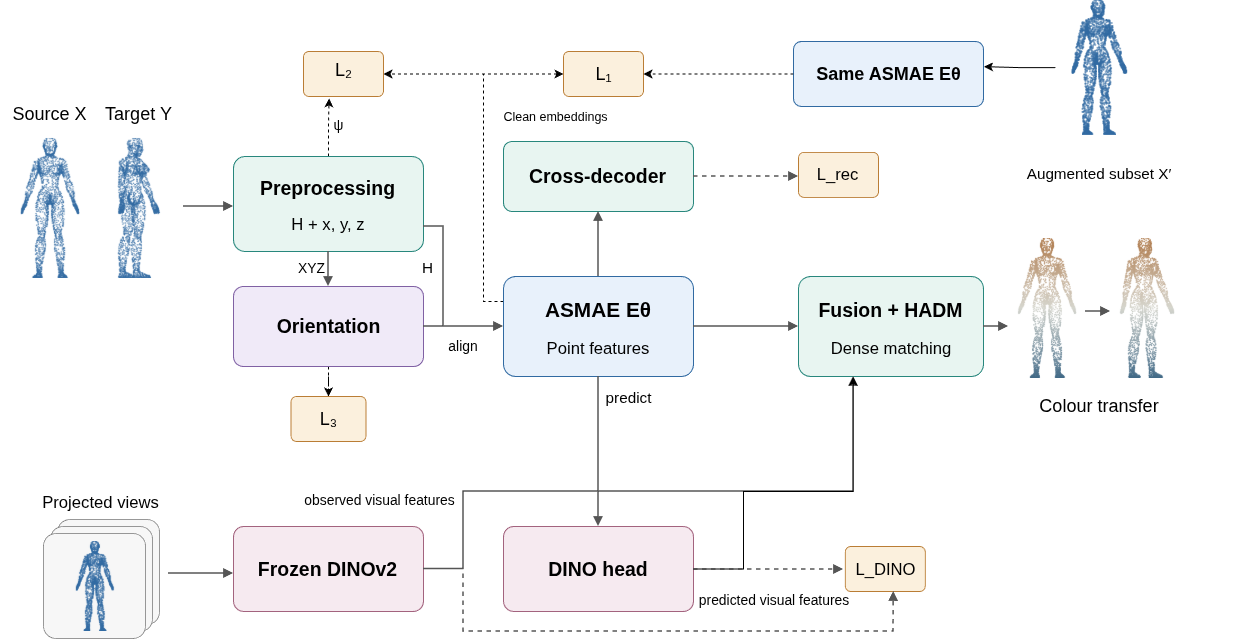
\includegraphics[width=\textwidth]{current/pipeline-overview.png}
\caption[Correspondence pipeline and training objectives.]{Correspondence pipeline and training objectives. Dashed connections identify supervision; solid connections show the flow of features and geometry. Here $L_1=L_{\mathrm{self}}$ is the self-identity objective; $L_2$ groups $L_{\mathrm{cycle}}$, $L_B$, $L_{\mathrm{orient}}$ and $L_{\mathrm{sep}}$; and $L_3$ groups the orientation objectives $L_{\mathrm{bin}}$, $L_{\mathrm{res}}$, $L_{\mathrm{subset}}$ and $L_{\mathrm{domain}}$. The colour-transfer pair illustrates how a dense point map transfers a source attribute to its corresponding target points.}
\label{fig:current-pipeline}
\end{figure}

\section{Point-Cloud Preprocessing}
\subsection{Surface points and neighbourhood graph}
The preprocessing module extracts vertex positions from the input shape and represents them as an unordered point cloud. Coordinates are centred and normalized to provide a consistent scale. A nearest-neighbour graph connects spatially nearby points, and its undirected adjacency matrix $A$ defines the graph Laplacian
\begin{equation}
 L=D-A,
\end{equation}
where $D$ is the diagonal degree matrix. Eigenpairs $(\lambda_\ell,\phi_\ell)$ describe variation over the graph and provide the spectral basis for the geometric descriptors. Figure~\ref{fig:preprocessing} shows the conversion from surface geometry to the input feature matrix.

\begin{figure}[H]
\centering
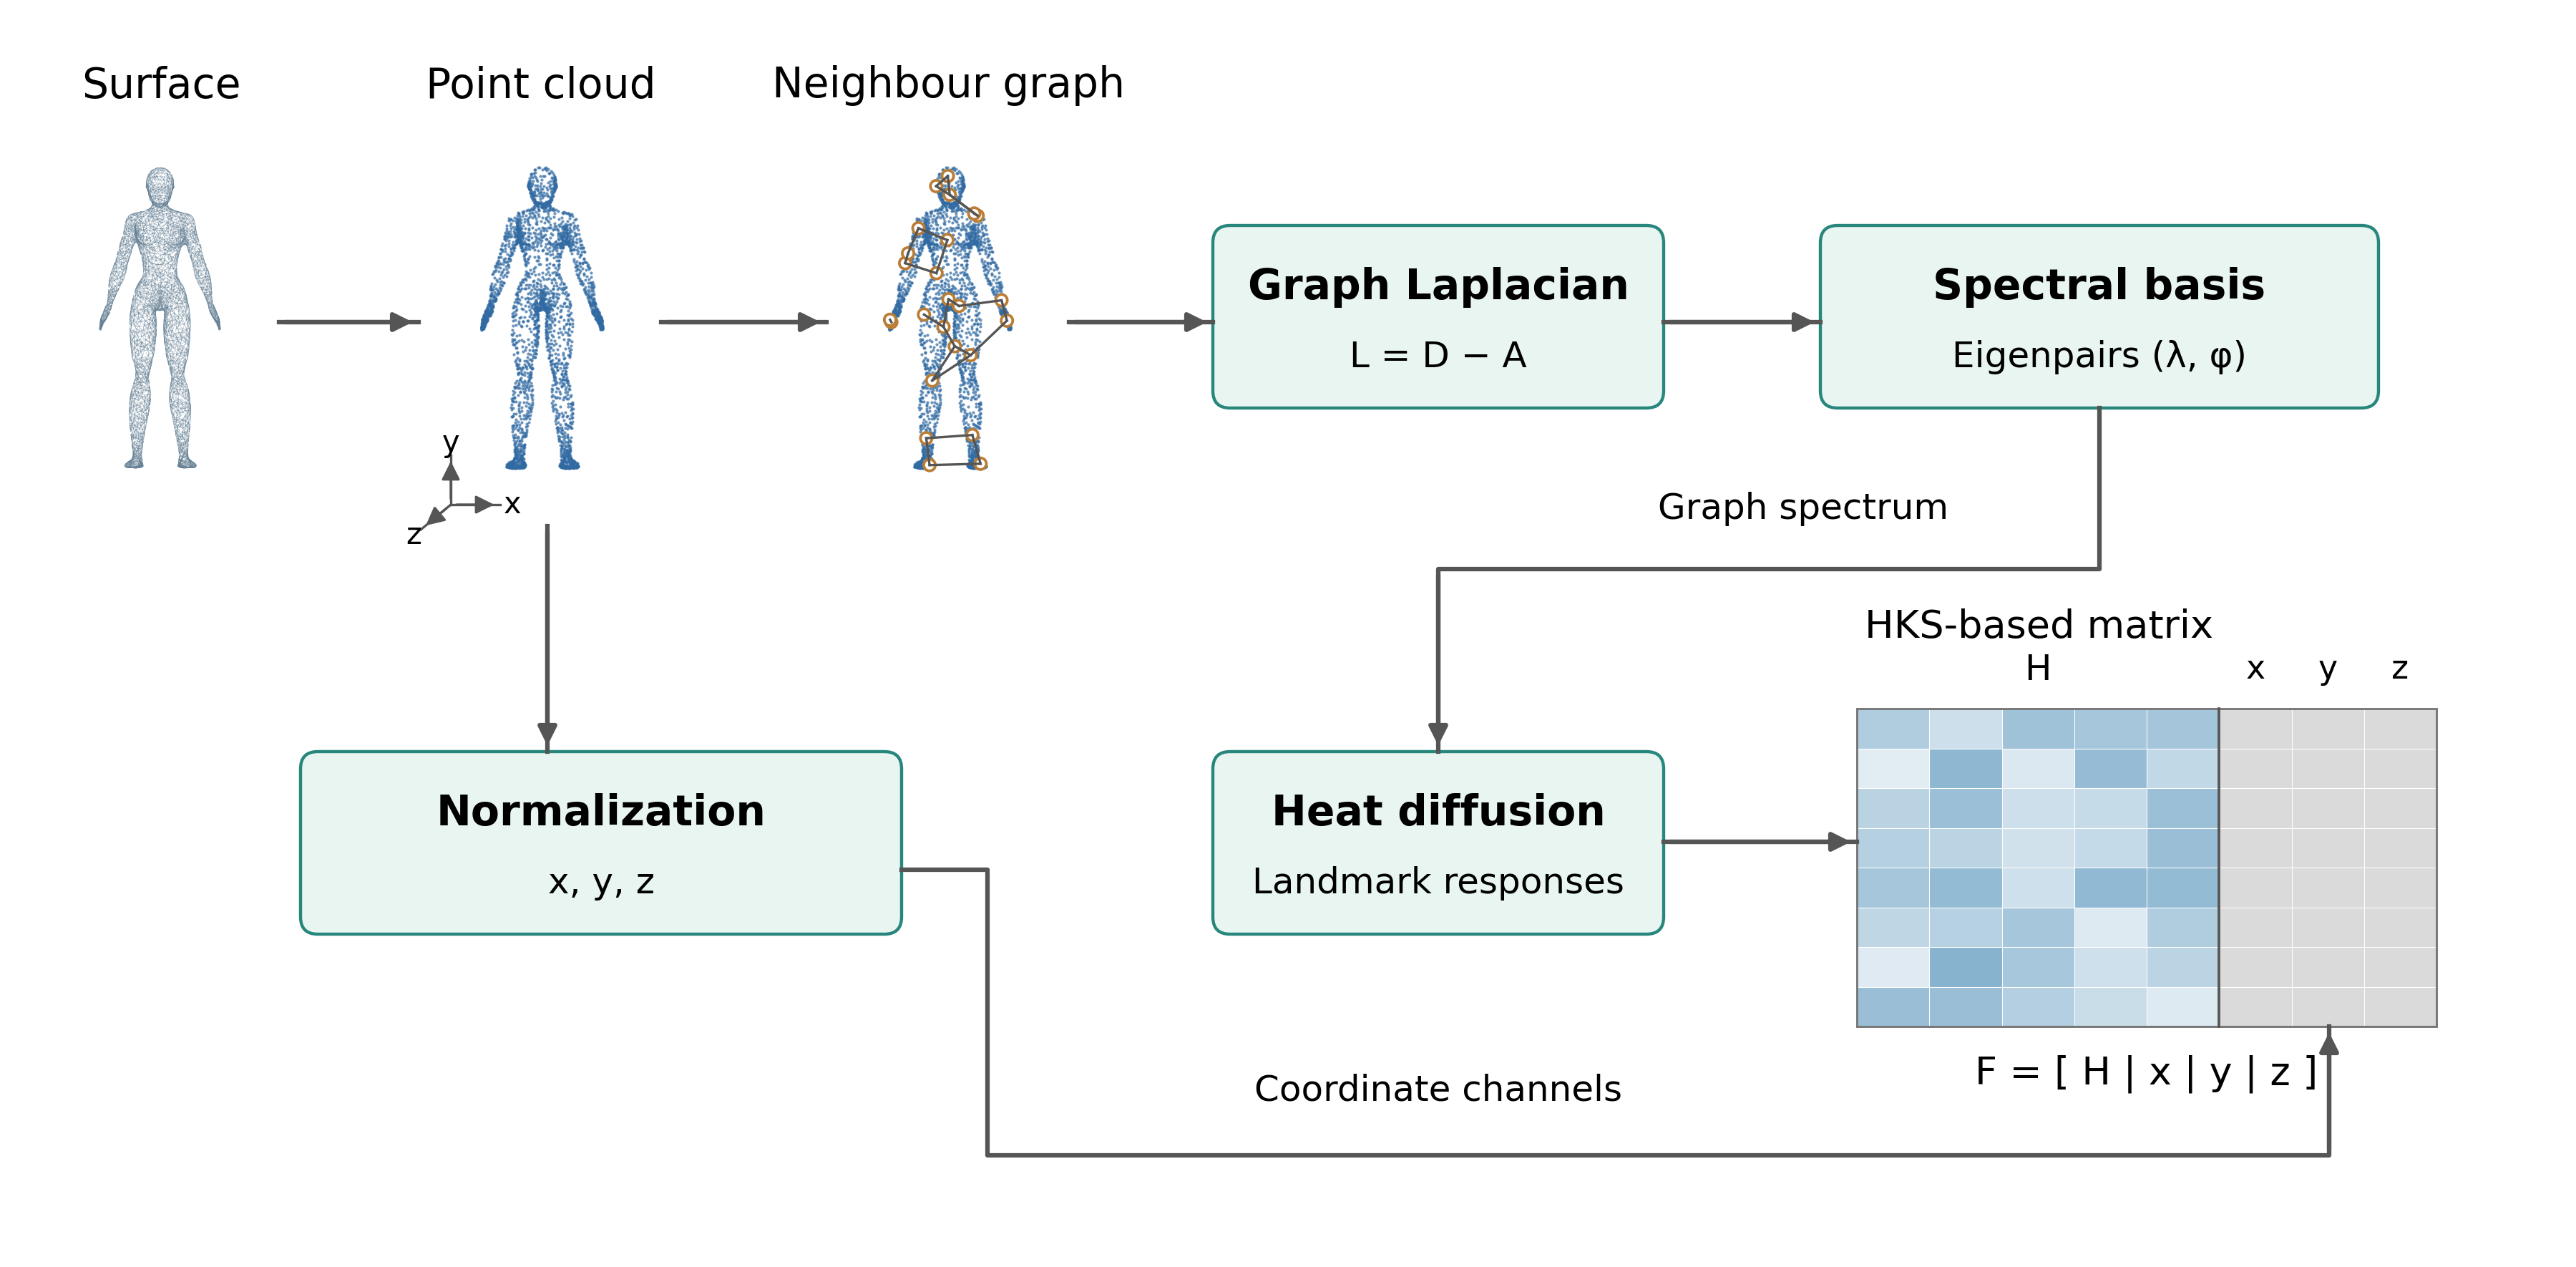
\includegraphics[width=\textwidth]{current/preprocessing.png}
\caption[Point-cloud and heat-descriptor preprocessing.]{Point-cloud and heat-descriptor preprocessing. Sampled surface positions form the point cloud and neighbourhood graph. The graph spectrum produces the heat-based descriptor matrix $H$, which is concatenated with normalized $x$, $y$ and $z$ coordinates. Matrix shading illustrates the organization of descriptor channels.}
\label{fig:preprocessing}
\end{figure}

\subsection{Heat descriptors and coordinate channels}
Heat diffusion describes how information spreads between locations on the graph. For sampled landmarks $s_1,\ldots,s_q$, the descriptor at point $x_i$ is
\begin{equation}
 H_{ij}=K_t(x_i,s_j)=\sum_\ell e^{-t\lambda_\ell}
 \phi_\ell(x_i)\phi_\ell(s_j).
\label{eq:landmark-heat}
\end{equation}
This HKS-based representation uses landmark heat responses \citep{10.5555/1735603.1735621}. Each row corresponds to a point, and each column records diffusion from a landmark. Channel normalization and logarithmic scaling balance the descriptor magnitudes.

The encoder input concatenates the heat matrix with explicit coordinates:
\begin{equation}
 F_X=[H_X\mid x\mid y\mid z].
\end{equation}
The coordinate channels supply position information alongside the spectral descriptor. They are expressed in the same frame as the point positions passed to the encoder. After relative alignment, the target coordinate channels are updated accordingly.

\subsection{Intrinsic geometric embedding}
A biharmonic embedding supplies distances for geometric regularization and anchor consistency \citep{Lipman_2010_Biharmonic}:
\begin{equation}
 \psi(x)=\left[\frac{\phi_1(x)}{|\lambda_1|},\ldots,
 \frac{\phi_r(x)}{|\lambda_r|}\right],\qquad
 d_B(x,x')=\|\psi(x)-\psi(x')\|_2.
\end{equation}
Nonzero spectral modes define the embedding, which is normalized by a reference distance scale. The resulting representation describes the relative separation of points through the graph geometry.

\section{Relative Orientation Module}
\subsection{Pairwise encoding and feature interaction}
The orientation estimation module (OEM) takes independently sampled subsets of the source and target. Shared point encoding extracts local features, and cross-shape feature interaction relates regions of one shape to the other. Global pooling produces a pair representation for predicting relative yaw about the vertical axis. The architecture follows the orientation-learning principle of SE-ORNet \citep{Deng_2023_CVPR}.

\begin{figure}[H]
\centering
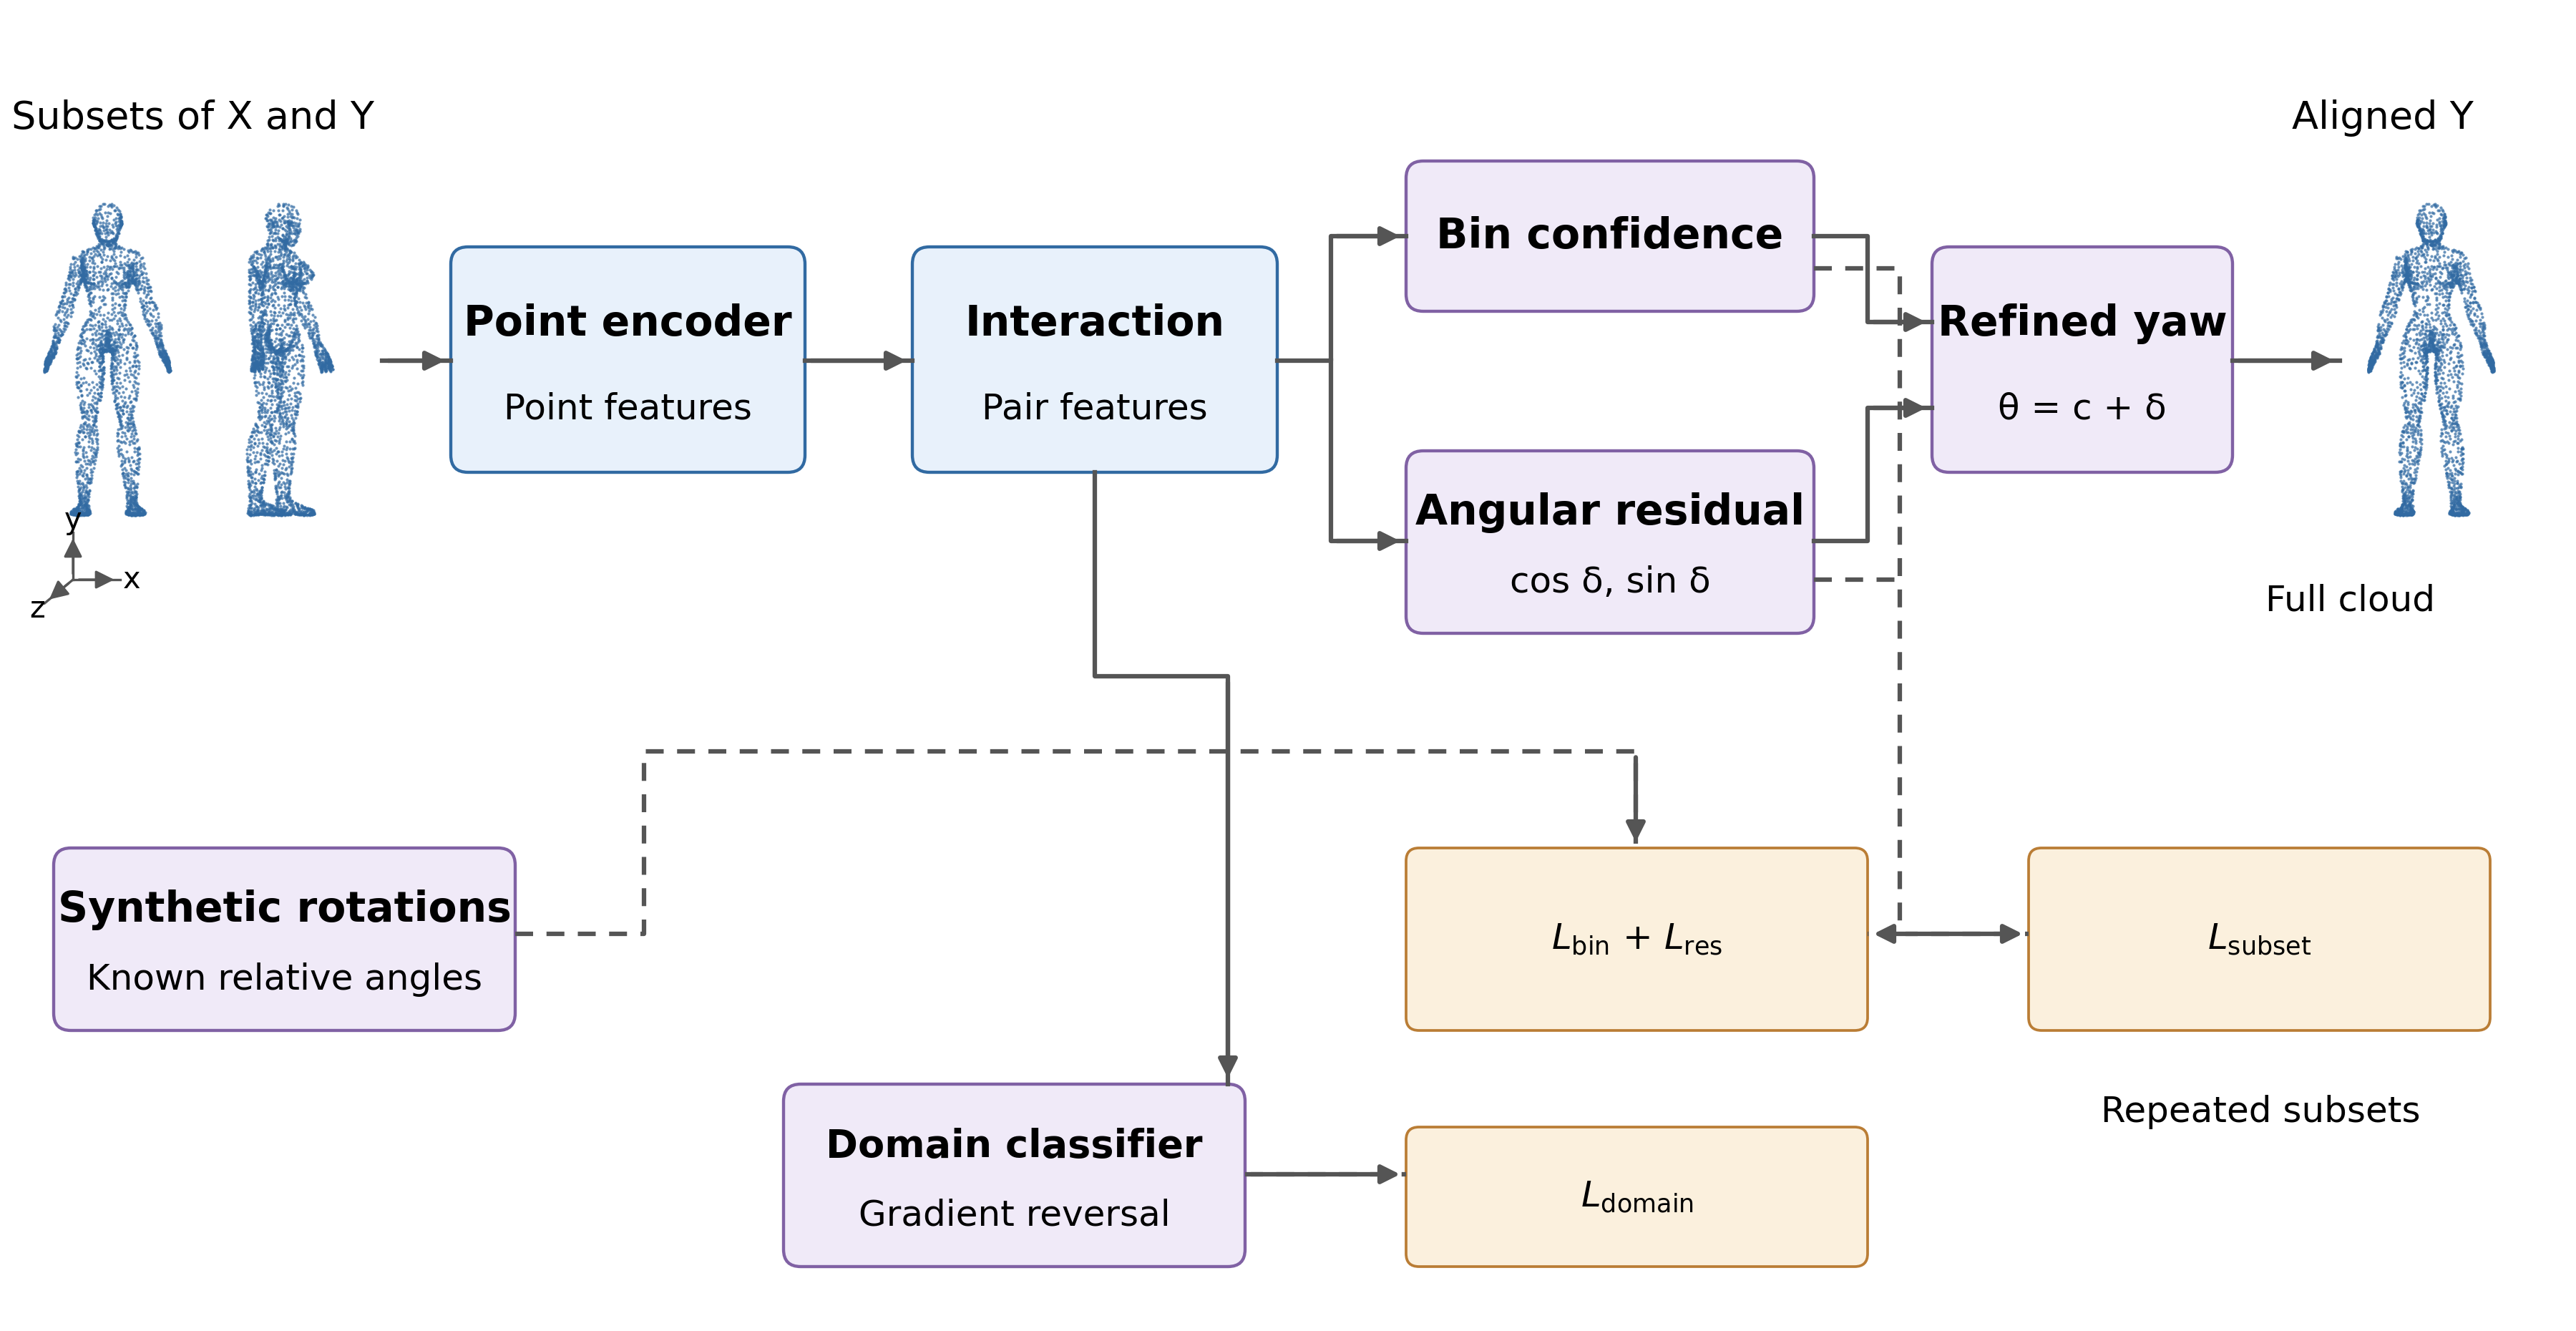
\includegraphics[width=\textwidth]{current/orientation-module.png}
\caption[Relative orientation estimation.]{Relative orientation estimation. Pairwise point features predict angular-bin confidence and a continuous residual. Synthetic rotations supervise angle prediction, repeated point subsets supply consistency supervision, and a domain discriminator connects synthetic and cross-shape pairs. The predicted yaw aligns the full target point cloud.}
\label{fig:orientation}
\end{figure}

\subsection{Continuous angular prediction}
Overlapping angular bins provide coarse orientation hypotheses. For each bin with centre $c_k$, the network predicts confidence $p_k$ and a normalized residual vector $r_k$. Following the MultiBin principle \citep{Mousavian_2017_MultiBin}, the residual represents the displacement from the bin centre through cosine and sine. The predicted angle is
\begin{equation}
 k^*=\arg\max_k p_k,\qquad
 \hat\theta=c_{k^*}+\operatorname{atan2}(r_{k^*,2},r_{k^*,1}).
\end{equation}
The residual supports continuous alignment between bin centres. Overlap allows a boundary angle to be represented by neighbouring bins. The inverse predicted rotation aligns all target points with the source frame.

\subsection{Orientation supervision}
Synthetically rotating a shape produces a paired observation with a known relative angle. Forward and inverse directions supervise the bin probabilities and residuals. Independently sampled observations of the same pair provide a consistency objective on both outputs. A gradient-reversal discriminator distinguishes synthetic same-shape pairs from cross-shape pairs \citep{JMLR:v17:15-239}; focal loss weights this domain classification \citep{Lin_2017_ICCV}.

The orientation objective combines angular classification, residual prediction, subset consistency and domain adaptation. Alignment is detached when supplying coordinates to the correspondence branch, so OEM is trained by its dedicated supervision while ASMAE is trained by representation objectives.

\section{ASMAE Representation Learning}
\subsection{Shared geometric encoder}
ASMAE maps the input heat descriptors and XYZ coordinates to point embeddings. A feature projection and a positional encoding initialize the point tokens. Local attention aggregates neighbouring tokens, with relative geometric direction supplying an attention bias. Both shapes pass through the same encoder parameters, placing their descriptors in a common feature space.

\begin{figure}[H]
\centering
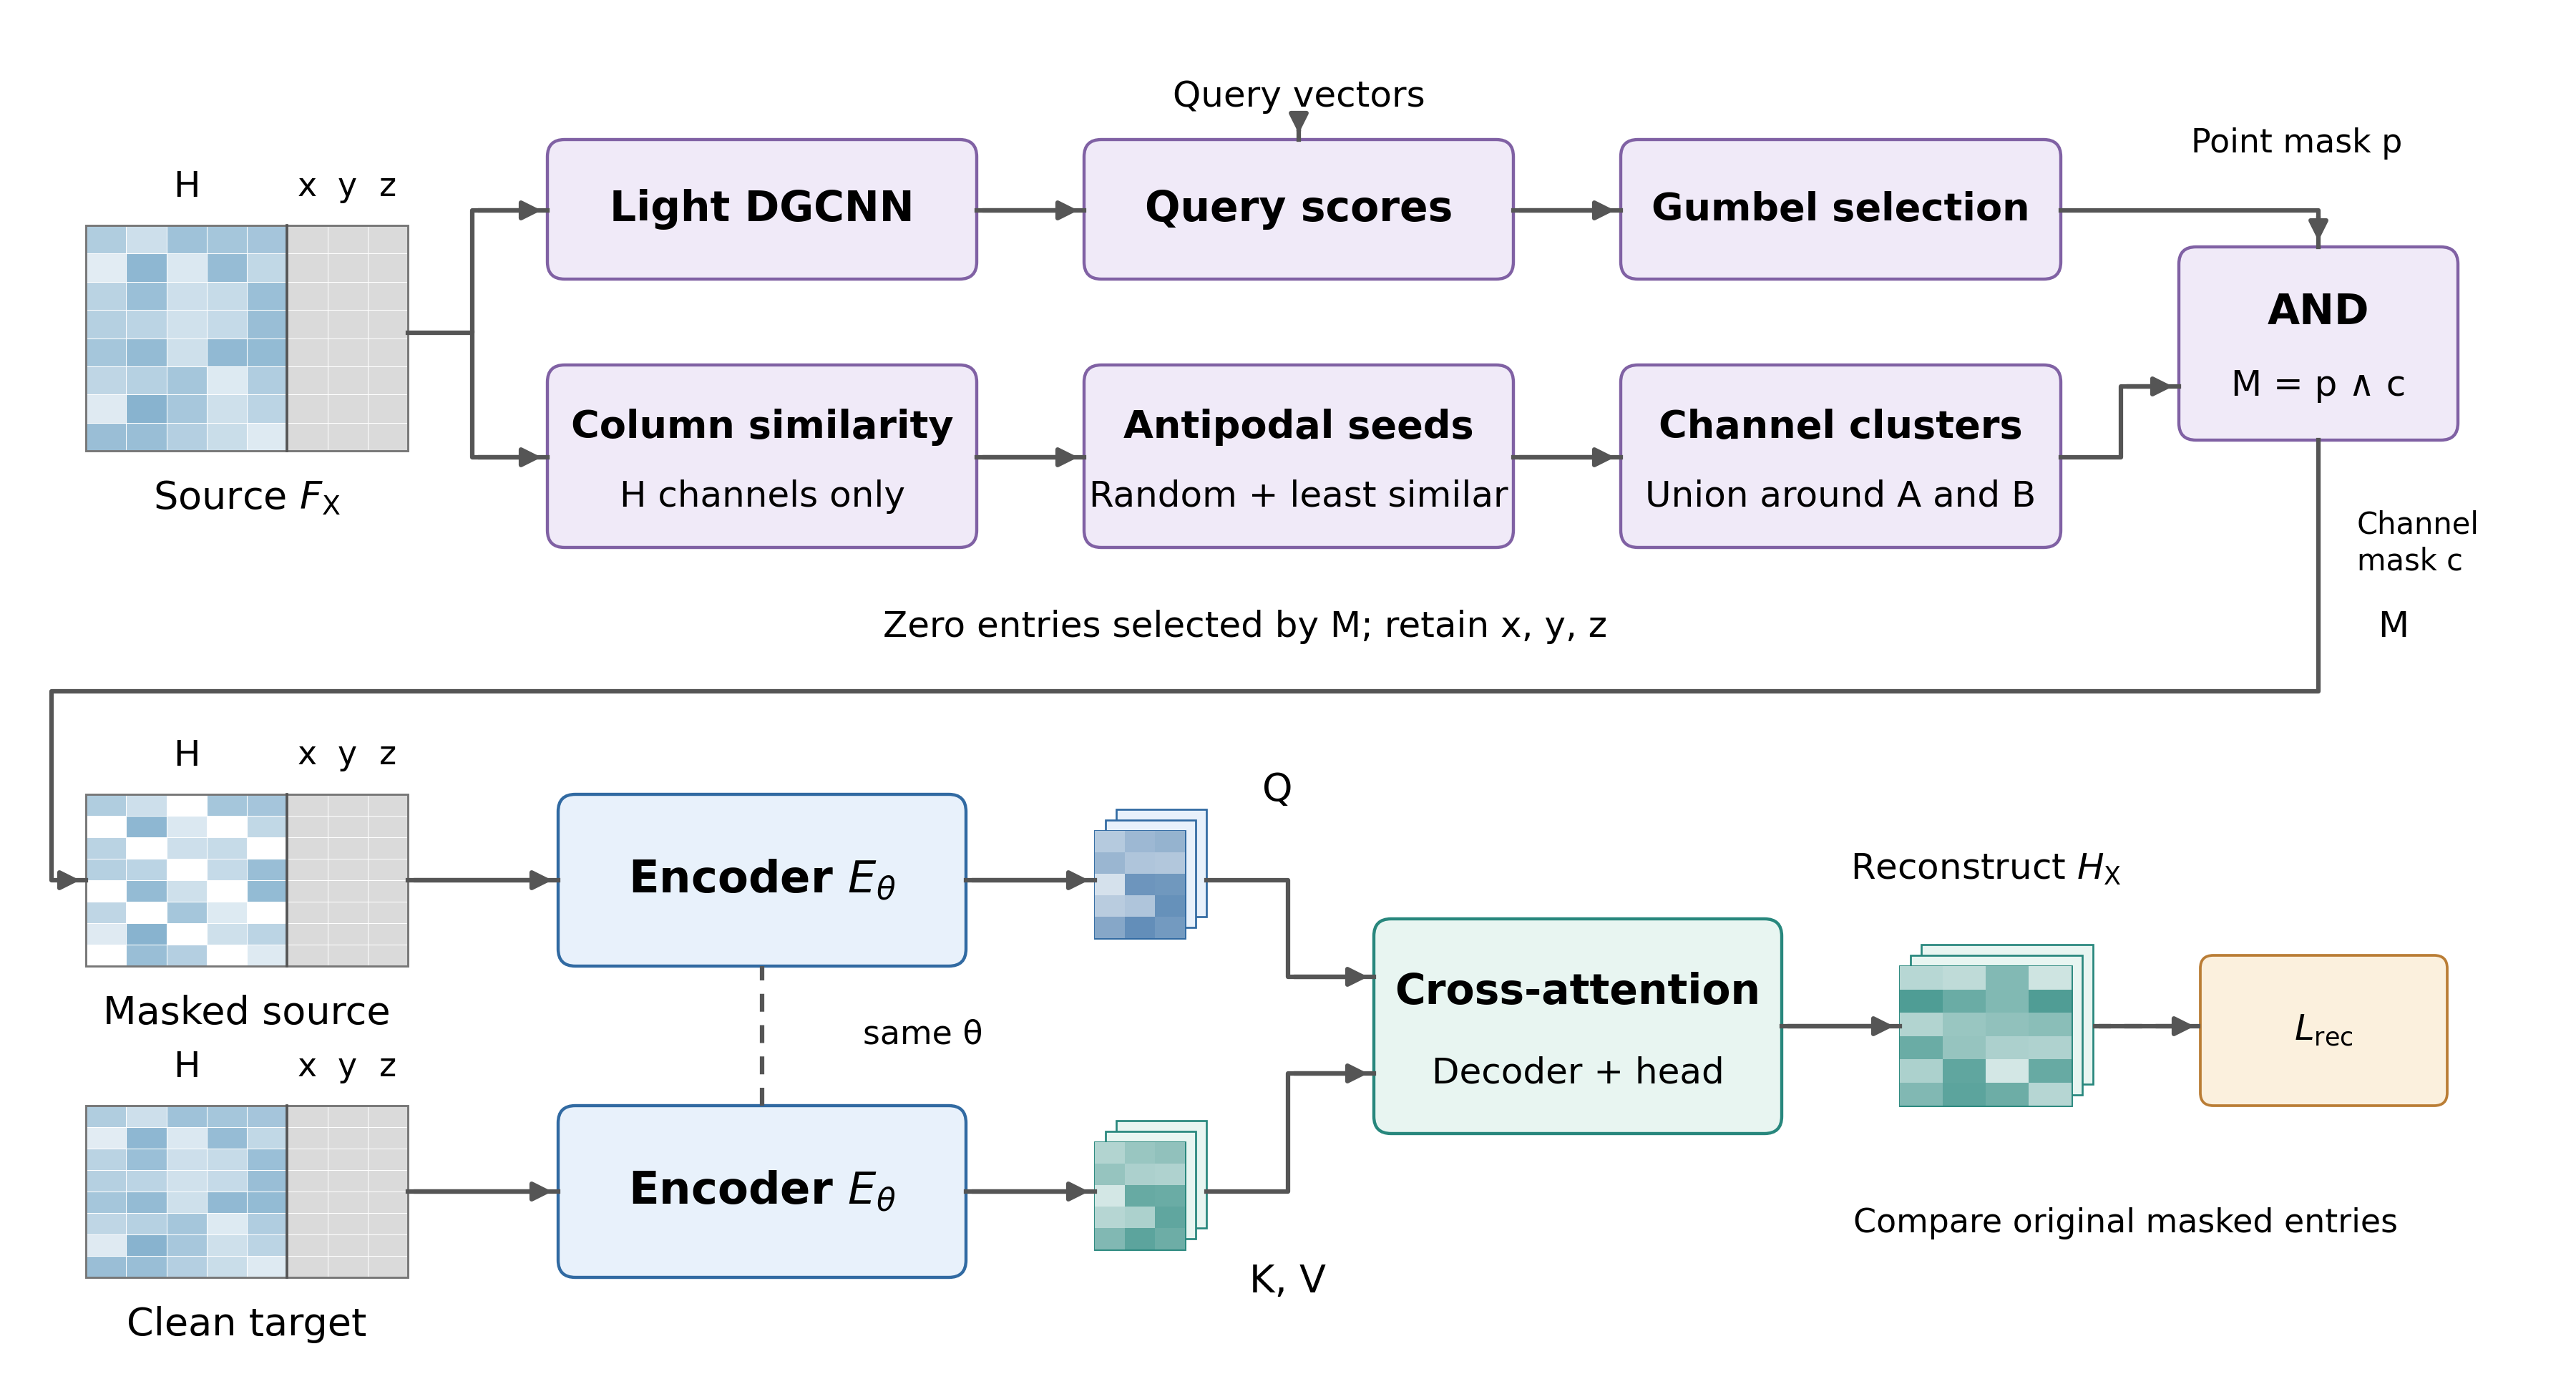
\includegraphics[width=\textwidth]{current/asmae-pipeline.png}
\caption[ASMAE with explicit coordinate conditioning.]{ASMAE and its mask generator. Point selection and descriptor-channel selection jointly define the mask; XYZ remains visible. Masked source tokens query clean target features for reconstruction, also performed in the reverse direction. Both $E_\theta$ blocks denote the same encoder parameters; the mask generator has its own Light DGCNN.}
\label{fig:asmae}
\end{figure}

\subsection{Descriptor masking and cross-reconstruction}
The AAMG mask generator has two selection branches, shown in Figure~\ref{fig:asmae}. A Light DGCNN extracts features for point selection. Query vectors score these features, and hard Gumbel selection chooses point locations. The union of selected locations gives a binary point mask $p_i$.

The second branch computes cosine similarity between descriptor columns, excluding XYZ. It selects a random seed channel and a channel least similar to that seed, then combines channels similar to each seed. This gives a channel mask $c_j$. Their intersection defines the entries to hide:
\begin{equation}
 M_{ij}=p_i\land c_j,\qquad
 \widetilde F_{ij}=\begin{cases}0,&M_{ij}=1,\\ F_{ij},&M_{ij}=0.\end{cases}
\end{equation}
Coordinate channels remain visible, and all point positions are retained. The Light DGCNN belongs to the mask generator; the shared ASMAE encoder $E_\theta$ processes the resulting masked or clean feature matrices.

The masked source representation supplies decoder queries. Clean target embeddings supply keys and values, allowing the decoder to use cross-shape context to reconstruct source descriptors. Exchanging the source and target gives bidirectional reconstruction. This paired masked-learning design is motivated by AMIGO \citep{article}. Separate clean encoder passes supply embeddings for the auxiliary objectives and matching.

\section{Visual Feature Module}
The visual branch projects the point cloud into multiple depth-based views. A frozen DINOv2 backbone extracts patch descriptors \citep{oquab2024dinov2learningrobustvisual}. Visibility testing associates image samples with surface points, and aggregation across views produces a point descriptor $d_i$ with observation confidence $c_i$. Neighbourhood smoothing shares visual context locally.

A prediction head maps each geometric embedding to a visual descriptor $\hat d_i$. Distillation weights the lifted observations by confidence:
\begin{equation}
 L_{\mathrm{DINO}}=
 \frac{\sum_i c_i\,[1-\cos(\hat d_i,d_i)]}{\sum_i c_i}.
\end{equation}
The objective is evaluated on both shapes. At matching time, observation confidence controls the blend of observed and predicted visual features. The visual branch therefore supplies both training supervision and an inference descriptor, following the use of lifted visual information in non-rigid matching \citep{Chen_2025_CVPR}.

\section{Representation Objectives}
\label{sec:objectives}
The representation objectives supervise complementary properties of the shared encoder. Reconstruction uses masked entries, geometric objectives use clean paired embeddings, self-identity uses an augmented observation of the same shape, and visual distillation uses lifted DINOv2 descriptors.

\subsection{Reconstruction and feature separation}
The reconstruction loss measures the absolute error on masked descriptor entries in both directions. A separation term discourages excessive similarity between distinct points. For normalized embeddings $z_i$, its form is
\begin{equation}
 L_{\mathrm{sep}}(Z)=\frac{1}{N(N-1)}\sum_{i\ne j}
 \max(z_i^\top z_j-m,0),
\end{equation}
where $m$ is the similarity margin. Together, these objectives preserve reconstructive information and discrimination between point features.

\subsection{Cycle and intrinsic consistency}
Feature similarities define directional soft maps
\begin{equation}
 P_{XY}=\operatorname{softmax}_{j}(Z_XZ_Y^\top/\tau),
\end{equation}
with temperature $\tau$. The reverse map is constructed analogously. The cycle objective measures coordinate recovery after mapping in both directions:
\begin{equation}
 L_{\mathrm{cycle}}=\operatorname{MSE}(P_{XY}P_{YX}X,X)
 +\operatorname{MSE}(P_{YX}P_{XY}Y,Y).
\end{equation}

For intrinsic consistency, the soft map transports the target biharmonic embedding to source indexing, $\widetilde\Psi_X=P_{XY}\Psi_Y$. The directional distortion is
\begin{equation}
 L_B(X,Y)=\underset{i,j}{\operatorname{mean}}
 \left|d_B^X(i,j)-\|\widetilde\psi_X(i)-\widetilde\psi_X(j)\|_2\right|.
\end{equation}
Averaging the two directions encourages matched points to preserve the intrinsic relationships within each shape.

\subsection{Local orientation consistency}
Neighbouring source points form triplets with directed area vectors. Their soft-mapped triplets define corresponding vectors in the aligned target frame. An angular agreement term compares the normalized vectors. This supplies a local directional constraint alongside the distance-based objective.

\subsection{Self-identity supervision}
The self-identity branch uses the same ASMAE encoder $E_\theta$ as reconstruction and clean feature extraction. It reuses the clean source embedding $Z_X=E_\theta(F_X,X)$ and computes an additional embedding for an augmented source subset. Both passes share parameters and receive gradients from the identity objective.

A clean shape and an augmented subset share point identities. Rotation, scaling and coordinate perturbations change the observation while retaining the correspondence of sampled vertices. An InfoNCE objective \citep{Oord_2018_CPC} treats the matching point as a positive candidate:
\begin{equation}
 L_{\mathrm{self}}=-\frac{1}{|Q|}\sum_{i\in Q}
 \log\frac{\exp(z_i^\top z'_{\pi(i)}/\tau_s)}
 {\sum_j\exp(z_i^\top z'_j/\tau_s)}.
\end{equation}
Here $Q$ contains queried source identities retained in the subset, $\pi(i)$ is the subset position of the same original vertex, and $\tau_s$ controls the contrastive distribution. Embeddings are normalized before comparison. Cross-entropy rewards the matching identity against all other points in the augmented subset. The objective is evaluated on the source member of each ordered training pair.

\subsection{Joint optimization}
Representation learning combines the objectives through weights $\lambda_j$:
\begin{equation}
 L_{\mathrm{rep}}=\sum_{j\in\mathcal J}\lambda_jL_j,
 \quad\mathcal J=\{\mathrm{rec,sep,cycle},B,\mathrm{orient,self,DINO}\}.
\end{equation}
Training first establishes relative orientation and then introduces the representation objectives progressively. The overall objective combines $L_{\mathrm{rep}}$ with OEM and domain supervision. This separates the supervision of alignment from the learning of point descriptors while connecting both through the aligned inputs.

\section{Heat-Anchored Deformation Matching}
\label{sec:hadm}
HADM converts geometric and visual embeddings into a dense point map through orientation selection, anchor propagation and deformation refinement.

\subsection{Orientation selection and feature fusion}
Predictions from independently sampled point subsets contribute orientation votes. Candidate alignments include strong angular modes and a half-turn alternative. For each candidate, the target is aligned and encoded. Intrinsic anchor agreement and feature similarity jointly score the candidate, and the selected alignment supplies the pair for refinement.

Observed and predicted visual descriptors are blended using their confidence. A shared dimensionality reduction places the visual features of both shapes in a common compact representation. Normalized geometric and visual feature blocks are then fused for correspondence search.

\subsection{Intrinsic anchor consistency}
Mutual feature matches propose anchor pairs. Similarity margins rank their confidence, while spatial coverage in biharmonic space distributes candidates across the shape. Agreement between candidate pairs is measured by
\begin{equation}
 W_{uv}=\exp\left[-\frac{
 (d_B^X(a_u,a_v)-d_B^Y(b_u,b_v))^2}{2\sigma_c^2}\right].
\end{equation}
A spectral score identifies mutually compatible candidates, and consistency filtering forms the anchor set. This uses the pairwise-compatibility principle of spectral matching \citep{Leordeanu_2005_Spectral}.

\subsection{Anchor propagation}
Corresponding anchors define proximity descriptors on both shapes:
\begin{equation}
 h_{j,\sigma}(x)=\exp\left[-\frac{
 \|\psi(x)-\psi(a_j)\|_2^2}{2\sigma^2}\right].
\end{equation}
These Gaussian responses encode position relative to the anchor set in biharmonic space. Combining them with point features transfers anchor information to other locations. Successive stages expand and refine the anchor set using this additional context.

\subsection{Deformation and dense assignment}
A similarity transformation estimated from the anchors initializes source alignment. A deformation graph then represents non-rigid adjustment through local node transformations \citep{10.1145/1275808.1276478}. Each point blends nearby transformations to obtain its deformed position. Positional agreement and anchor constraints guide the fit, while as-rigid-as-possible regularization encourages compatible motion between neighbouring graph nodes \citep{sorkine2007rigid}. Refinement proceeds from a coarse graph to finer spatial detail.

The final map combines fused feature similarity with deformed positional agreement:
\begin{equation}
 T(i)=\arg\max_j\left[G_X(i)^\top G_Y(j)
 -\lambda_p\|\widetilde x_i-y_j\|_2^2\right].
\end{equation}
Here $G$ contains the fused features and anchor-relative descriptors, and $\widetilde X$ is the deformed source. The resulting point indices support attribute transfer between shapes, as illustrated by the colour-transfer operation in Figure~\ref{fig:current-pipeline}.
 
\chapter{Experiments and Results}
\label{Chapter4}
\lhead{Chapter 4. \emph{Experiments and Results}}

\section{Datasets}
FAUST \citep{Bogo_2014_FAUST}, SCAPE \citep{10.1145/1186822.1073207}, SHREC'19 \citep{Melzi_2019_SHREC} and SURREAL \citep{Varol_2017_SURREAL} provide human-shape data for studying correspondence under variation in pose and identity. FAUST contains registered human scans, SCAPE models articulated body deformation, SHREC'19 addresses correspondence between human shapes, and SURREAL supplies synthetic human observations. These benchmarks connect geometric matching to the anatomical structure of deformable bodies.

\section{Correspondence Evaluation}
For a source point $i$, let $T(i)$ be its predicted target and $T^*(i)$ the reference match. Normalized geodesic error measures their separation on the target surface:
\begin{equation}
 e_i=\frac{d_Y(T(i),T^*(i))}{\sqrt{\operatorname{area}(Y)}}.
\end{equation}
The mean over evaluated vertices gives a pair score, and averaging pair scores gives the aggregate error. Lower error indicates closer agreement with the reference correspondence. Surface-area normalization supports comparison across different shape scales.

Colour transfer provides a complementary view of the dense map. A source colour field assigns distinct colours to different regions, and correspondence transfers these attributes to the target. Consistent placement of colour regions allows inspection of anatomical alignment across changes in pose. The same visualization convention supports comparisons between the pipeline and its component variants.

% Editorial insertion point: verified quantitative comparison tables and measured
% colour-transfer results for the pipeline and ablations. These comments do not
% render in the report. Do not insert illustrative outputs as experimental evidence.
 
\chapter{Conclusion}
\label{Chapter5}
\lhead{Chapter 5. \emph{Conclusion}}

This report presents a correspondence pipeline that connects point-cloud representation learning with relative orientation and deformation-guided matching. Spectral heat descriptors capture relationships over the point graph, while explicit XYZ channels provide coordinate context. The orientation module places the input pair in a compatible frame using angular classification and continuous refinement.

The shared ASMAE learns point features through masked reconstruction across the two shapes. Geometric consistency preserves spatial relationships, self-identity supervision retains point identity under augmentation, and DINOv2 distillation transfers visual information to the geometric representation. These objectives connect local discrimination with shape-wide structure.

HADM combines geometric and visual features to propose correspondences, identifies anchors through intrinsic consistency, and propagates their information across the shapes. Deformation refinement then links the feature representation to positional agreement. The resulting dense point map provides the basis for transferring surface attributes between differently posed shapes.

The experimental progression highlights the complementary roles of representation, orientation and matching. Distortion regularization partially reduced left--right ambiguity in qualitative inspection, while front--back ambiguity motivated relative orientation modelling. The resulting design uses a shared encoder, continuously refined alignment and anchor-guided deformation as connected modules of the correspondence system.

\section{Ablation Overview}
\label{sec:ablation-overview}
The experimental progression examines the representation, alignment and matching components of the correspondence pipeline. The following observations summarize the motivation for each group of experiments, with detailed descriptions in Appendix~\ref{app:development}.

The initial student--teacher baseline studied correspondence learning without explicit geometric descriptors. A moving-average teacher supplied consistency targets to the student. The baseline and its reconstruction formulation are described in Section~\ref{app:baseline}.

Adding XYZ coordinates supplied positional context alongside the point descriptors. Protecting these channels during masking retained a spatial reference for reconstruction. Section~\ref{app:coordinates} explains coordinate conditioning and its connection to the choice of reference frame.

DINOv2 introduced a complementary visual cue through descriptors lifted from projected views. This experiment examined visual feature matching before the later distortion and orientation changes; its construction is described in Section~\ref{app:dino}.

Distance-preservation regularization reduced left--right ambiguity to some extent in qualitative inspection. Front--back ambiguity motivated the subsequent directional and alignment experiments. Section~\ref{app:distortion} describes the distortion objective and these observations.

The descriptor experiments combined heat-based features, WKS and normals estimated from point-cloud neighbourhoods. These were point-estimated normals, not mesh normals. Section~\ref{app:descriptors} discusses the complementary spectral and directional information.

Canonicalization explored a shared reference frame before correspondence estimation. Relative orientation then used pairwise feature interaction through the SE-ORNet orientation module. These approaches are detailed in Sections~\ref{app:canonical} and~\ref{app:oem}, respectively.

The orientation variants examined coordinate noise, independently sampled points, arbitrary-angle augmentation and boundary avoidance. Overlapping bins and continuous residuals supplied a finer angular representation. Sections~\ref{app:robustness} and~\ref{app:refinement} describe these experiments and subset consistency.

The shared-encoder design removed the student--teacher arrangement following observed degradation and combined intrinsic distortion, self-identity supervision and visual distillation. HADM connected the features to anchor consistency and deformation refinement. Section~\ref{app:hadm} describes this integration.


%----------------------------------------------------------------------------------------
%	BIBLIOGRAPHY
%----------------------------------------------------------------------------------------
%\nocite{*}

\lhead{\emph{Bibliography}} % Change the page header to say "Bibliography"

\nocite{*} % Include all references in the Bibliography, even if not cited in the text

\bibliographystyle{apalike} % Use the "custom" BibTeX style for formatting the Bibliography

\clearpage
\phantomsection
\addcontentsline{toc}{chapter}{Bibliography}
\label{Bibliography}
\bibliography{Bibliography} % The references (bibliography) information are stored in the file named "Bibliography.bib"

\clearpage
\appendix
\chapter{Experimental Development}
\label{app:development}
\lhead{Appendix A. \emph{Experimental Development}}

This appendix explains the experimental progression summarized in Section~\ref{sec:ablation-overview}. The variants examine how representation, orientation and geometric matching interact when estimating correspondence between deformable shapes.

\section{Student--Teacher Baseline}
\label{app:baseline}
The initial experiment used student--teacher learning without explicit geometric descriptors. The student learned from paired shape observations, and a moving-average teacher supplied a consistency target. This follows the broader principle of stabilizing representation learning through a slowly updated target model \citep{NIPS2017_68053af2}.

Masked reconstruction related the source to a reference shape. The associated global matching objective used an entropically regularized transport formulation \citep{Cuturi_2013}. This stage established a representation-learning baseline for examining the contribution of additional geometric and visual cues.

\section{Adding Coordinates}
\label{app:coordinates}
Explicit XYZ channels introduced positional information into the point representation. Coordinates describe the location of a point within the shape and complement spectral descriptors that can be similar at symmetric locations. The input matrix combined heat-based features with normalized spatial coordinates.

Coordinate conditioning also made the reference frame relevant to feature learning. The same anatomical point can change its coordinates under rotation, and different poses can place corresponding body parts in different positions. This connection between position and orientation motivated the alignment experiments. Protecting coordinate channels during masking preserved the positional context of hidden descriptor entries.

\section{Adding DINOv2 Features}
\label{app:dino}
The visual-cue experiment added DINOv2 features to the matching representation \citep{oquab2024dinov2learningrobustvisual}. Projected shape views supplied image descriptors, which were lifted to their visible points. Aggregation across views associated each point with visual context complementary to the geometric encoder.

This stage focused on adding the visual cue before the later distortion and orientation changes. Visibility handling controlled which image observations contributed to a point descriptor. The feature-matching path combined the lifted representation with learned point features. Visual distillation, described later, extended this connection into the training objectives.

\section{Distortion and Symmetry}
\label{app:distortion}
A distance-preservation objective constrained the spatial relationships induced by a soft correspondence. If $P$ maps source indices to target points, the transported positions are $\widehat Y=PY$. The Euclidean distortion objective compares distances between source points and their transported counterparts:
\begin{equation}
 L_{\mathrm{dist}}=\underset{i,j}{\operatorname{mean}}
 \left|\|x_i-x_j\|_2-\|\widehat y_i-\widehat y_j\|_2\right|.
\end{equation}

In qualitative inspection, this term corrected left--right ambiguity to some extent. It encouraged groups of matched points to preserve their spatial relationships, rather than making each assignment independently. Front--back ambiguity then became a central focus: a large region could have coherent matches while being associated with the opposite facing direction. The following experiments examined additional directional cues and explicit orientation estimation.

\section{HKS, WKS and Point Normals}
\label{app:descriptors}
A richer geometric representation combined heat-based features, WKS, coordinates and normal components. HKS and WKS describe complementary aspects of the spectrum \citep{10.5555/1735603.1735621,Aubry_2011_WKS}. Normal components supplied a local directional cue alongside these descriptors.

The normals were estimated from point-cloud neighbourhoods; they were not mesh normals. Local covariance analysis identified the direction of least variation as a normal axis. Centroid-based orientation and neighbourhood sign propagation supplied variants for assigning its direction. The normal and coordinate channels were preserved during reconstruction masking.

The experiments also examined an orientation penalty based on normal compatibility and a global proper-rotation criterion based on a fitted transformation. Reflecting the coordinate frame provided another way to examine front--back and left--right alternatives. These variants connected local descriptors with the direction implied by a candidate correspondence.

\section{Canonical Orientation}
\label{app:canonical}
Canonicalization predicted a common frame for each shape before matching. A global point-cloud representation produced a continuous rotation parameterization \citep{Zhou_2019_CVPR}, which was converted to an orthonormal transformation and applied to the centred points. Synthetic rotations supplied a known relationship between transformed observations.

Equivariance, canonical-coordinate agreement and consistency supervision encouraged the same shape to retain a common canonical interpretation under rotation. The approach is related in purpose to shape--pose disentanglement \citep{Katzir_2022_ShapePose}. The experiments highlighted the importance of choosing compatible frames across different articulated poses, motivating pairwise relative orientation.

\section{SE-ORNet Orientation Estimation}
\label{app:oem}
The pairwise orientation module estimates how the target is rotated relative to the source. Cross-shape feature interaction connects the two point representations before angular prediction. The SE-ORNet formulation \citep{Deng_2023_CVPR} supplied the foundation for synthetic rotation supervision and domain adaptation.

A synthetically rotated copy of a shape supplies known forward and inverse angles. Real pairs of distinct shapes contribute to domain adaptation, which aligns their pair representations with those of synthetic observations. Group normalization \citep{Wu_2018_GroupNorm} stabilizes intermediate feature normalization. The estimated relative rotation is applied before coordinate-conditioned correspondence learning.

The orientation experiments also examined the relationship between learning alignment and learning correspondence. Orientation-focused optimization established the alignment task before progressively introducing the representation objectives. This separates their supervision while connecting their outputs through the aligned point coordinates.

\section{Noise, Sampling and Angular Boundaries}
\label{app:robustness}
\subsection{Coordinate noise and point sampling}
Coordinate perturbations tested orientation learning under small changes in the observed positions. Scaling perturbations by cloud size made them relative to the input geometry. Independently sampled point subsets tested whether the pair representation retained the same orientation information when different points were observed.

Random sampling and spatially distributed sampling provided complementary subset strategies. The orientation prediction was applied to the full target cloud, preserving all points for dense correspondence. Reconstruction masking addressed a different question: it hid feature information while retaining the point locations and coordinate context for ASMAE.

\subsection{Arbitrary angles and boundary avoidance}
Angle-centre training associated synthetic rotations with discrete orientation classes. Arbitrary-angle augmentation extended the observations between class centres, exposing the classifier to continuously varying orientations. A boundary-avoidance variant restricted training rotations to neighbourhoods of the bin centres, excluding the regions where adjacent class assignments change.

These experiments separated two issues: sensitivity to class boundaries and quantization of a continuous angle. Avoiding boundary regions altered the training distribution, while continuous residual prediction supplied an explicit way to represent the displacement within a bin.

\section{Continuous Angular Refinement}
\label{app:refinement}
The refinement experiment combined overlapping angular bins with a residual for each bin, following MultiBin \citep{Mousavian_2017_MultiBin}. A confidence score selected an orientation hypothesis, and a cosine--sine vector described its continuous correction. Overlapping support allowed nearby bins to share supervision for boundary angles.

Independent observations of the same pair supplied subset consistency. The objective compared their bin distributions and the residual predictions associated with corresponding bins. This retained separate orientation hypotheses while encouraging agreement under point resampling. Multiple subset predictions also supplied votes during inference.

\section{Shared Representation and HADM}
\label{app:hadm}
The student--teacher arrangement was removed after it was observed to degrade correspondence during development. A shared ASMAE model learned both shapes directly, and the associated global transport objective was removed in the same redesign. Reconstruction was combined with intrinsic distortion, self-identity supervision and visual distillation.

Biharmonic distortion compares distances in a spectral embedding \citep{Lipman_2010_Biharmonic}. Self-identity supervision associates the same vertices across augmented observations through an InfoNCE objective \citep{Oord_2018_CPC}. DINOv2 distillation transfers lifted visual information into the learned point representation, with observation confidence weighting the contribution of each point.

HADM connects these representations to geometric matching. Fused features propose anchors, intrinsic distance agreement filters the proposals, and anchor-relative descriptors propagate spatial context. Orientation hypotheses are evaluated using feature and anchor evidence. A deformation graph then refines source positions under data, anchor and local rigidity constraints \citep{10.1145/1275808.1276478,sorkine2007rigid}. Dense assignment combines the resulting positional agreement with feature similarity. This integration links relative alignment, representation learning and non-rigid refinement within a single correspondence pipeline.

\backmatter

\end{document}  
